\documentclass{article} % Especially this!

\usepackage[english]{babel}
\usepackage[utf8]{inputenc}
\usepackage[margin=1.5in]{geometry}
\usepackage{amsmath}
\usepackage{amsthm}
\usepackage{amsfonts}
\usepackage{amssymb}
\usepackage{graphicx}
\usepackage[siunitx]{circuitikz}
\usepackage{tikz}
\usepackage[colorinlistoftodos, color=orange!50]{todonotes}
\usepackage{hyperref}
\usepackage[numbers, square]{natbib}
\usepackage{fancybox}
\usepackage{epsfig}
\usepackage{soul}
\usepackage[framemethod=tikz]{mdframed}
\usepackage[shortlabels]{enumitem}
\usepackage[version=4]{mhchem}
\usepackage{multicol}
\usepackage{graphicx}
\graphicspath{ {./} }

\newcommand{\blah}{blah blah blah \dots}

\setlength{\marginparwidth}{3.4cm}

\newcommand{\summary}[1]{
\begin{mdframed}[nobreak=true]
\begin{minipage}{\textwidth}
\vspace{0.5cm}
\end{minipage}
\end{mdframed}}

\renewcommand*{\thefootnote}{\fnsymbol{footnote}}

\title{
\normalfont \large
\textsc{ASSIGNMENT-3
\vspace{10pt}
\\COL 216, Spring 2021} \\
[10pt] 
\rule{\linewidth}{0.5pt} \\[6pt] 
\Large Interpreter for MIPS Assembly Language Instructions \\
\rule{\linewidth}{2pt}  \\[10pt]
}
\author{Jitender Kumar Yadav, 2019CS10361
\\Asha Ram Meena, 2019CS10337}
\date{\normalsize March 13, 2021}
\begin{document}

\maketitle
\section{Problem Statement}
\textbf{Develop an interpreter for a subset of MIPS assembly language instructions.}

\section{Algorithm and Approach}
A MIPS assembly file interpreter for files containing the following instructions was designed in C++: add, sub, mul, beq, bne, slt, j, lw, sw and addi. The memory, register contents, instructions etc. were stored in internal data structures and the program would validate the file for syntax errors and output the hexadecimal register contents and the number of clock cycles and executions.
\begin{itemize}
    \item[$\diamond$] The file containing the instructions is read from the given location and the syntax is checked while storing the instructions in the memory.
    \item[$\diamond$] The instructions are read line by line and the corresponding memory changes are checked and tasks like load, store, addition and subtraction are performed as per need.
    \item[$\diamond$] The data in the 32 registers is stored in an array and so is the auxiliary memory containing $2^{20}$ bits.
    \item[$\diamond$] The operations keep on updating the memory and register contents along side. The register contents are hexadecimal quantities.
    \item[$\diamond$] In case of any wrong memory is accessed by the assembly program, the program returns an error.
    \item[$\diamond$] The registers may be accessed by using MIPS conventions \$s and \$t or by integers 1-32.
\end{itemize}

\section{Input and Output}
\subsection{Input Specifications:}
\begin{itemize}
    \item The input is a single string containing the name of the text file, storing the .text part of the MIPS instructions containing syntactically correct instructions involving the above mentioned commands.
\end{itemize}
\subsection{Output}
\begin{itemize}
    \item The output is a set of printed lines in command lines. The first few lines print the hexadecimal values of the contents of the registers R0-R32 after each statement is evaluated.
    \item The last two lines print the no of clock cycles and the number of times each instruction has been executed as comma separated values.
\end{itemize}
\subsection{Sample I/O}
    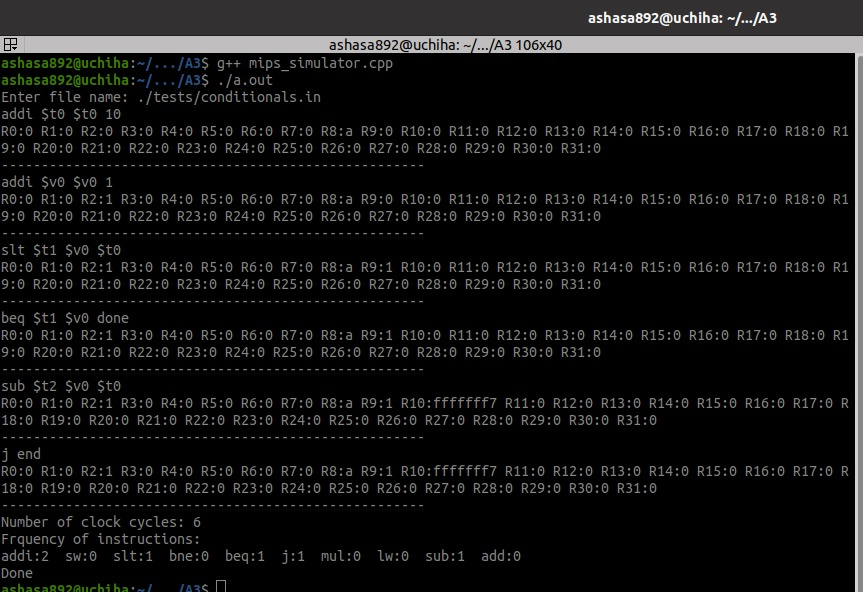
\includegraphics[scale = 0.45]{sampleio_A3.JPG}

\section{Testing}
A few test cases were generated to test the Simulator. These have been stored in the directory A3\_TestCases as text files containing the required portion of the asm code.

\end{document}